\documentclass[tikz]{standalone}

\usepackage{amsmath}
\usepackage{physics}

\usetikzlibrary{arrows.meta,backgrounds,fit,positioning}

\begin{document}
	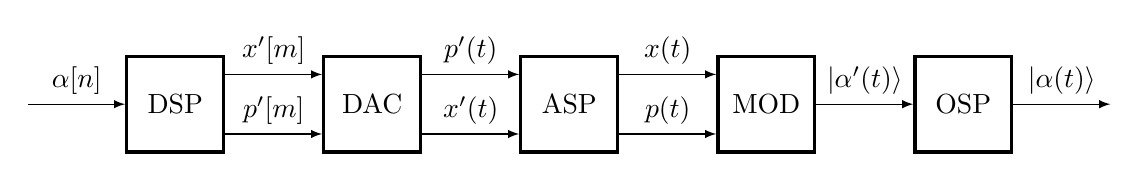
\begin{tikzpicture}[
		node distance=3.5em,
		arrow/.style={-latex},
		block/.style={draw, very thick, fill=white, minimum height=8ex, minimum width=3.5em},
	]
		\coordinate (in) at (0,0);
		\node (dsp) [block, right=of in] {DSP};
		\node (dac) [block, right=of dsp] {DAC};
		\node (asp) [block, right=of dac] {ASP};
		\node (mod) [block, right=of asp] {MOD};
		\node (osp) [block, right=of mod] {OSP};
		\coordinate[right=of osp] (out);
		
		\draw[arrow] (in) -- (dsp) node[midway, above]{$\alpha[n]$};
		\draw[arrow] ([yshift=2.5ex]dsp.east) -- ([yshift=2.5ex]dac.west) node[midway, above]{$x^\prime[m]$};
		\draw[arrow] ([yshift=-2.5ex]dsp.east) -- ([yshift=-2.5ex]dac.west) node[midway, above]{$p^\prime[m]$};
		\draw[arrow] ([yshift=-2.5ex]dac.east) -- ([yshift=-2.5ex]asp.west) node[midway, above]{$x^\prime(t)$};
		\draw[arrow] ([yshift=2.5ex]dac.east) -- ([yshift=2.5ex]asp.west) node[midway, above]{$p^\prime(t)$};
		\draw[arrow] ([yshift=2.5ex]asp.east) -- ([yshift=2.5ex]mod.west) node[midway, above]{$x(t)$};
		\draw[arrow] ([yshift=-2.5ex]asp.east) -- ([yshift=-2.5ex]mod.west) node[midway, above]{$p(t)$};
		\draw[arrow] (mod) -- (osp) node[midway, above]{$\ket{\alpha^\prime(t)}$};
		\draw[arrow] (osp) -- (out) node[midway, above]{$\ket{\alpha(t)}$};
	\end{tikzpicture}
\end{document}
